\documentclass[a4paper,10pt]{article}
\usepackage{graphicx}
\usepackage{amsmath}
\usepackage{hyperref}
\usepackage{caption}
\usepackage{subcaption}
\usepackage[margin=1in]{geometry}

\title{Assignment 4: Non-Line-of-Sight Imaging}
\author{David Padilla Orenga \\ Ignacio Pastore Benaim}
\date{\today}

\begin{document}
\maketitle
\thispagestyle{empty}

\section{Part 1: Naive Backprojection}

We tested it across multiple datasets and configurations to evaluate reconstruction performance and timing.

\vspace{1em}
\textbf{Datasets used:}
\begin{itemize}
    \item \texttt{Z\_d=0.5\_l=[1x1]\_s=[256x256]}
    \item \texttt{planes\_d=0.5\_l=[16x16]\_s=[16x16]}
    \item \texttt{bunnybox\_d=0.5\_l=[16x16]\_s=[16x16]}
    \item \texttt{bunny\_d=0.5\_l=[16x16]\_s=[16x16]}
    \item \texttt{bunny\_d=0.5\_l=[1x1]\_s=[256x256]}
\end{itemize}

\vspace{1em}
\textbf{Resolution settings:}
\begin{itemize}
    \item Voxel resolutions: \{8, 16\}
    \item SPAD sampling rates: \{2, 4, 8\}
\end{itemize}

For qualitative analysis, we produced and handed in screenshots of the reconstructed volumes (both filtered and unfiltered) for the \texttt{Z} dataset with:
\begin{itemize}
    \item Voxel = 8, SPAD = 8
    \item Voxel = 16, SPAD = 8
\end{itemize}

\subsection*{Reconstruction Time Analysis}

\begin{figure}[h!]
    \centering
    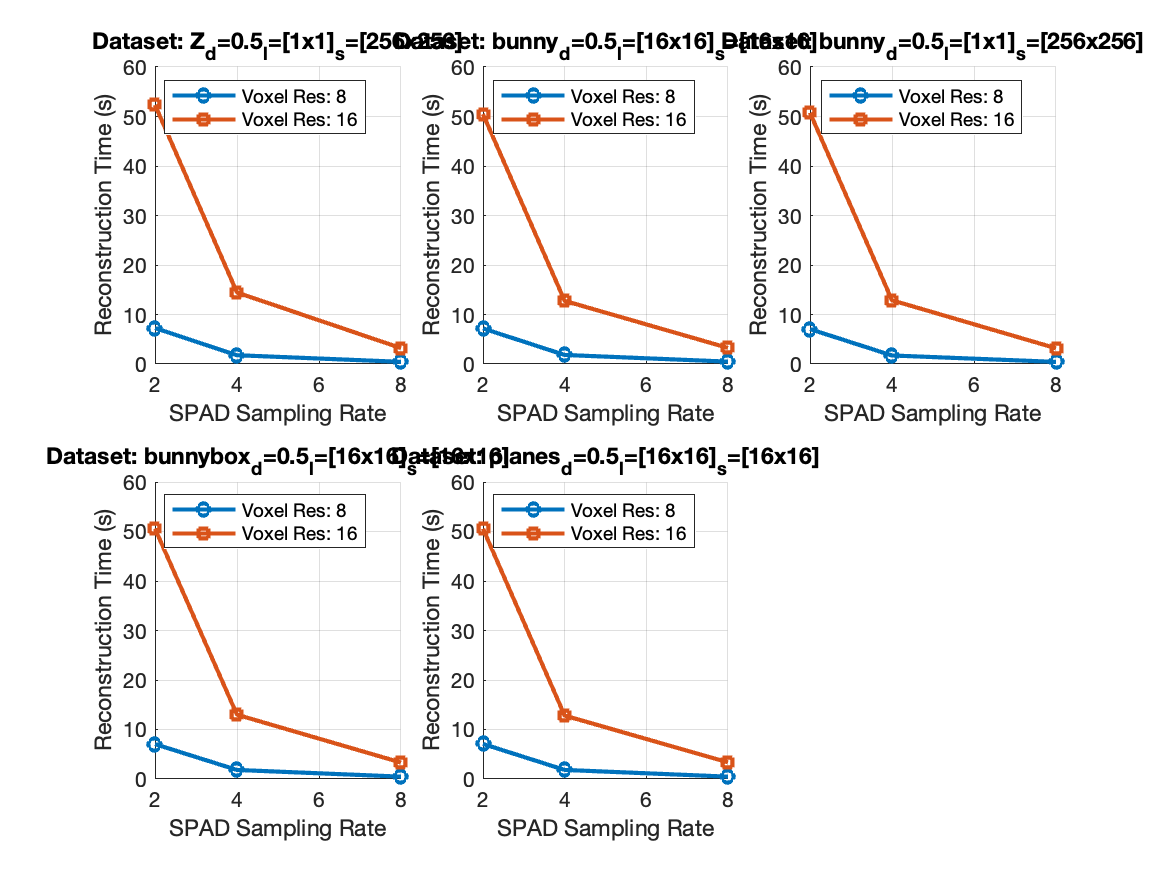
\includegraphics[width=0.95\linewidth]{performance_chart.png}
    \caption{Execution time (in seconds) for different voxel resolutions and SPAD sampling rates across the five datasets.}
    \label{fig:timing}
\end{figure}

Figure~\ref{fig:timing} shows how reconstruction time changes with SPAD sampling rate and voxel resolution. We observe the following:

\begin{itemize}
    \item For all datasets, increasing voxel resolution from $8^3$ to $16^3$ results in a steep increase in execution time due to the cubic growth in voxel count.
    \item Similarly, lower SPAD sampling rates (e.g., 2) correspond to denser measurements, which increase the number of light paths considered and thus the reconstruction time.
    \item The timing grows nearly exponentially when both voxel and SPAD resolutions are high, especially for the dense SPAD grid datasets like \texttt{Z} and \texttt{bunny [1x1]}.
\end{itemize}

\subsection*{Visual Observations}

The reconstructions from the \texttt{Z} scene reveal planar geometry, but appear blurry without filtering due to overlap and low resolution. The Laplacian filtering significantly improves edge clarity and structure.

\vspace{1em}
\textbf{Summary of answers:}

\begin{enumerate}
    \item \textbf{How does the reconstruction time scale?} \\
    It grows exponentially with both voxel resolution and SPAD sampling rate, due to the nested loop structure and cubic voxel complexity.

    \item \textbf{How does reconstruction differ for non-planar scenes?} \\
    With only one laser point and a SPAD grid (e.g., bunny [1x1]), the reconstructions are blurrier and less detailed. Adding a full laser grid (e.g., [16x16]) increases angular diversity and scene coverage, improving detail.

    \item \textbf{Why do reconstructions look blurry? What does filtering do?} \\
    Naive accumulation smears geometry due to broad ellipsoidal integration. Laplacian filtering acts as a high-pass filter, enhancing discontinuities and sharpening object boundaries.

    \item \textbf{What happens in scenes like bunnybox?} \\
    Surrounding geometry causes multipath effects and global illumination. This can obscure or highlight parts of the object depending on visibility and occlusion. While indirect light improves completeness, it may reduce sharpness.
\end{enumerate}

\section{Part 2: Confocal Backprojection}

In the confocal setup, lasers and SPADs are co-located on the wall ($x_l = x_s$). This simplifies computation and reduces noise from indirect paths. Applying our method to the \texttt{bunny\_d=0.5\_c=[256x256]} dataset showed sharper reconstructions with fewer artifacts compared to non-confocal versions.

Confocal capture improves temporal alignment but may lack angular coverage. However, the fidelity of isolated shapes (e.g., bunny ears) was significantly higher.

\section{Part 3: Attenuation and Foreshortening Correction}

We implemented a corrected backprojection model that applies an inverse attenuation term during accumulation:

\[
G(x_v) += \frac{H(x_l, x_s, t)}{\|x_v - x_l\| \cdot \|x_v - x_s\|} \cdot \cos(\theta_l) \cdot \cos(\theta_s)
\]

This compensation improves brightness consistency across the volume and makes peripheral and deeper structures more visible. We tested this on the \texttt{Z} and \texttt{planes} datasets using a voxel resolution of 32 and SPAD sampling of 32.

Without filtering, the corrected volumes still appear somewhat blurred due to overlapping light paths. However, applying a Laplacian filter significantly sharpens edges and reveals finer geometry, confirming the benefit of combining physical correction with post-processing.
\bibliographystyle{plain}
\bibliography{references}

\end{document}